\documentclass[a4paper,10pt,twocolumn]{article}

% =======================
% Packages
% =======================
\usepackage{amsmath, amssymb, amsthm, physics}
\usepackage{graphicx}
\usepackage{caption}
\captionsetup{font=small}
\usepackage{subcaption}
\usepackage{hyperref}
\usepackage{geometry}
\usepackage{float}
\usepackage{gensymb}
\usepackage{booktabs}
\usepackage{fancyhdr} % For custom headers/footers
\usepackage{indentfirst}
\usepackage[numbers]{natbib}  % if you want to control options explicitly
\setcitestyle{numbers,square}

\geometry{left=1.5cm, right=1.5cm, top=1.785cm, bottom=2.0cm}
\setlength{\parindent}{0in}
\sloppy

% =======================
% Header / Footer
% =======================
\pagestyle{fancy}
\fancyhf{}                     
\lhead{Computational Lab Report}
\rhead{Angze Li (CID: 02372394)}
\cfoot{\thepage}

\makeatletter
\let\ps@plain\ps@fancy        
\makeatother
% =======================
% Title
% =======================
\title{\textbf{Computational Lab Report: \\
Liquid Simulation}}
\author{Angze Li, CID: 02373494 \\
    Department of Chemistry, Imperial College London}

\begin{document}

\maketitle

% =========================================================
\section{Introduction}  % ~20\% of total marks, limit to ~1.5 page

\subsubsection*{Give a brief account on what molecular dynamics is, and what it aims to achieve. [5]}

Molecular dynamics (MD) is a computational technique used to study the motion and interactions of particles over time~\cite{leimkuhler2015molecular}. Since its development in the 1960s, MD has become one of the most widely used methods for predicting the behaviour and thermodynamic properties of solids, liquids, and gases. 

Broadly speaking, MD aims to achieve quantitative modelling and analysis of many-particle systems at the atomic scale. In an MD simulation, Newton’s equations of motion are numerically integrated for all particles in the system using an interatomic potential that describes the forces between them. Lennard--Jones (LJ) potential has been widely adopted in computing the interatomic potential due to its simple expression and good fit with experimental values. This calculation produces time-dependent trajectories for the positions and velocities of all atoms.

From these trajectories, a wide range of physical properties can be computed, including structural quantities such as radial distribution functions, dynamical properties such as diffusion coefficients and velocity autocorrelation functions, and thermodynamic quantities such as temperature, pressure, and energy~\cite{van1990computer}. Under the assumption of ergodicity, time averages obtained from sufficiently long MD trajectories are equivalent to ensemble averages~\cite{cho1992ergodicity}. In this way, MD enables the prediction of macroscopic behaviour from microscopic interactions through statistical mechanical averaging over the simulated trajectories.


\subsubsection*{Give two examples of instances where molecular dynamics simulations have/can be used (in a helpful way) instead of or in synergy with experimental techniques. In each case explain why. [10]}

MD has been widely adopted in the exploration of the conformational analysis of protein molecules due to the technical difficulties of probing marcomolecules experimentally. One of the most important applications is the study of protein folding~\cite{karplus2005molecular,swope2004describing,sugita1999replica}, which involves thermodynamics, kinetics, and
structure prediction. This is of great significance as the misfolding of proteins would lead to a range of diseases~\cite{dobson2003protein}. Though in the majority of the cases, simplified models needs to be applied for computationally efficient calculation, key aspects of the nature of protein folding can still be captured deterministically to find the trajectories of protein folding, thus providing the spatial and temporal resolution to investigate the biomolecules. 

A well-known example is the folding of the villin headpiece subdomain~\cite{lei2010folding}, which has been extensively studied using MD simulations due to its relatively small size and fast folding kinetics. MD simulations have been able to reproduce folding pathways and identify intermediate conformations, providing detailed atomistic insight into the mechanisms of protein folding that are difficult to capture experimentally. In combination with experimental techniques such as NMR spectroscopy~\cite{mcknight1997nmr} and kinetic measurements~\cite{zhu2011evidence}, MD simulations help to reveal the microscopic processes underlying protein stability and folding dynamics.

Quantitative transport and thermodynamic properties of ionic liquids (IL) have also been studied extensively by MD methods~\cite{maginn2007atomistic,cadena2006molecular}, where the MD trajectories can be obtained deterministically. ILs are defined as salts that are liquid below 100℃~\cite{cadena2006molecular}. The tunable chemical properties and non-volatile nature of ILs lead to a huge potential in various areas, including catalysis and synthesis~\cite{rogers2002ionic,steinrueck2015ionic}. Due to the ionic nature of the ILs, the physical properties can be changed drastically with relatively modest change in the chemical structure and constitutions of the ions. However, exploring ILs with ``brute force'' would be inefficient and time-consuming when there are numerous candidates for cations and anions. Therefore, MD can serve as a computational tool to better understand and predict the properties, accelerating the design of IL to meet specific requirements.

A well-studied example is the ionic liquid 1-butyl-3-methylimidazolium hexafluorophosphate ([bmim][PF$_6$]), which has been extensively investigated using molecular dynamics simulations. MD simulations have been used to calculate structural properties such as radial distribution functions as well as transport properties including diffusion coefficients and viscosity~\cite{raju2009aqueous}. These results have been compared with experimental measurements, helping to elucidate the microscopic origin of the unusually high viscosity and strong ion pairing observed in many ionic liquids~\cite{zhao2008shear}. In this way, MD simulations provide atomistic insight into ion organisation and dynamics, enabling the rational design of ionic liquids with tailored physical properties.


\subsubsection*{Computer simulations are performed under specific ``experimental'' conditions. The thermodynamic ensemble defines these conditions. Explain what is meant by the thermodynamic ensemble. Your answer should also provide three ensemble examples and briefly discuss what quantities are conserved in each ensemble. [5]}

A statistical ensemble is an idealised collection of a very large number of imaginary replicates of the system of interest~\cite{atkins2023atkins}. Thermodynamic properties are obtained by averaging over all possible microstates in the ensemble, where more probable states contribute more strongly to the ensemble average.

Three most commonly used ensembles in MD are the microcanonical (NVE), canonical (NVT) and grand canonical ($\mu$VT) ensemble. The microcanonical ensemble assumes that all the systems have the same energy, so they can be considered isolated. The number of particles ($N$), volume ($V$)and energy of the system are conserved for microcanonical ensemble. The canonical ensemble assumes that all the systems have the same temperature, while the system can exchange heat with a thermal reservoir, allowing the energy to fluctuate. The composition, volume and temperature of the system are conserved for canonical ensemble. Grand canonical allows particle  exchange, though chemical potentials are conserved. The chemical potential, volume and temperature of the system are conserved for grand canonical ensemble.

% =========================================================
% 2. Exercises / Results & Discussion (~60%)
% =========================================================
\section{Results and Discussion} % ~60\%

\subsection{Introduction to molecular dynamics simulation}
\subsubsection*{By taking Taylor expansions of $x(t+\delta t)$ and $x(t-\delta t)$, write general expressions for them up to the fourth order $\mathcal{O}(t^4)$. Having written these expressions, derive the formula in Figure 2 used to update positions in the classical Verlet algorithm: $x_i(t+\delta t)\approx2x_i(t)-x_i(t-\delta t)+\frac{F_i(t)}{m}\,\delta t^2$ by using Newton’s second law to replace $\frac{d^2 x_i(t)}{dt^2}$. [4 marks]}

For a function $f(x)$ that is infinitely differentiable at $a$, Taylor expansion is defined as:
\[
f(a+\delta x)=\sum_{n=0}^{+\infty}\frac{f^{(n)}(a)}{n!}(\delta x)^n.
\]
Let $x_i(t+\delta t)$ denote the position of an arbitrary atom $i$ at time $t+\delta t$. Expanding $x_i(t+\delta t)$ up to the fourth order gives:
\[
x(t+\delta t)=x(t)+x'(t)\delta t+\frac{x''(t)}{2}(\delta t)^2+\frac{x'''(t)}{6}(\delta t)^3+\mathcal{O}(t^4).
\]
Since $x'(t)=v(t)$ and $x''(t)=a(t)$,
\[
x(t+\delta t)=x(t)+v(t)\delta t+\frac{a(t)}{2}(\delta t)^2+\frac{a'(t)}{6}(\delta t)^3+\mathcal{O}(t^4).
\]
Substituting $\delta t$ by $-\delta t$, we obtain
\[
x(t-\delta t)=x(t)-v(t)\delta t+\frac{a(t)}{2}(\delta t)^2-\frac{a'(t)}{6}(\delta t)^3+\mathcal{O}(t^4).
\]
Adding $x(t-\delta t)$ to $x(t+\delta t)$ gives
\[
x(t+\delta t)+x(t-\delta t)=2x(t)+a(t)(\delta t)^2+\mathcal{O}(t^4).
\]
Using Newton's law ($F(t)=ma(t)$) and omitting $\mathcal{O}(t^4)$, the equation becomes
\[
x(t+\delta t)+x(t-\delta t)\approx2x(t)+\frac{F(t)}{m}(\delta t)^2.
\]
By rearranging, we arrive at
\[
x(t+\delta t)\approx 2x(t)-x(t-\delta t)+\frac{F(t)}{m}(\delta t)^2,
\]
which is the formula used in the classic Verlet algorithm (CVA,~\cite{verlet1967computer}).

\subsubsection*{What could be an advantage of the Velocity-Verlet algorithm over the classical Verlet algorithm? [2 marks]}

The Velocity-Verlet algorithm (VVA,~\cite{swope1982computer}) lets us calculate the atom velocities explicitly by using
\[
v_i(t+\delta t)=v_i(t+\frac{1}{2}\delta t)+\frac{1}{2}a_i(t+\delta t)\delta t.
\]
Though when VVA is adopted, we need to specify the initial velocities apart from the initial positions, this algorithm comes with several advantages compared to the CVA. A number of physical, especially dynamical quantities depend on velocity, e.g., kinetic energy, temperature, where VVA allows accurate calculation of these quantities at each timestep without approximation. Additionally, while retaining the same global error, stochastic collisions of atoms can easily be implemented for the VVA algorithm as velocities are computed for the entire trajectory.~\cite{andersen1983rattle}

\subsubsection*{Consider the Lennard-Jones pair potential. What physical interaction(s) does it describe? What is the physical significance for the $r^{-6}$ and $r^{-12}$ terms? [3 marks]}
\begin{figure}[H]
    \centering
    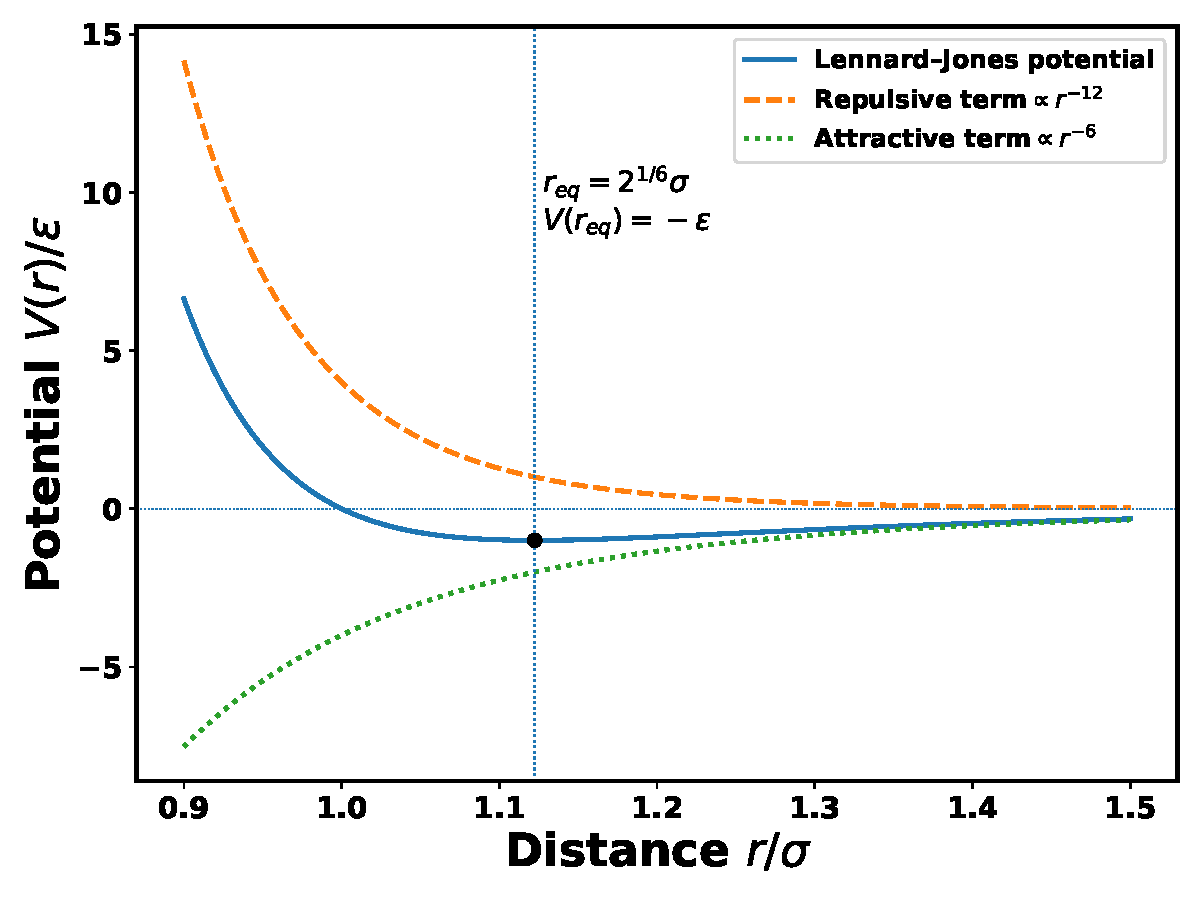
\includegraphics[width=1\linewidth]{Figures/lj_potential.pdf}
    \caption{Lennard–Jones potential showing the short-range repulsive $r^{-12}$ term and long-range attractive $r^{-6}$ dispersion interaction. The potential minimum occurs at $r_{eq}=2^{1/6}\sigma$, where the energy is $V(r_{eq})=-\varepsilon$. The well depth $\varepsilon$ represents the interaction strength between two particles.}
    \label{fig:lj_potential}
\end{figure}
The LJ pair potential describes the interaction between two neutral atoms or molecules through a combination of attractive and repulsive forces. It was first proposed in 1924 to describe the cohesive energy of crystals of noble gases,~\cite{jones1924determination} and has since been widely used to model intermolecular interactions in simple liquids and gases.~\cite{wang2020lennard}

The attractive $r^{-6}$ term represents long-range London dispersion (van der Waals) interactions arising from instantaneous dipole–induced dipole correlations between particles. The repulsive $r^{-12}$ term models the strong short-range repulsion that occurs when electron clouds overlap, which is primarily a consequence of the Pauli exclusion principle. The behaviours of the potential from the two terms at different distances are shown in Fig.~\ref{fig:lj_potential}.

The depth of the potential well, $\varepsilon$, represents the strength of the interaction between two particles and corresponds to the minimum potential energy at the equilibrium separation. Physically, it reflects the cohesive energy scale of the interaction and determines how strongly particles are bound in the system.

\subsubsection*{For a single Lennard--Jones interaction, $\phi(r)=4\varepsilon\left[\left(\frac{\sigma}{r}\right)^{12}-\left(\frac{\sigma}{r}\right)^6\right]$, find the separation $r_0$ at which the potential energy is zero. What is the force at this separation? Find the equilibrium separation $r_{\mathrm{eq}}$ and determine the well depth $\phi(r_{\mathrm{eq}})$. Evaluate the integrals $\int_{2\sigma}^{\infty}\phi(r)\,dr$, $\int_{2.5\sigma}^{\infty}\phi(r)\,dr$, and $\int_{3\sigma}^{\infty}\phi(r)\,dr$ when $\sigma=\varepsilon=1.0$.
[4 marks]}

Let $\phi(r)=0$, dividing both sides by $4\varepsilon$ and moving repulsive term to the RHS, we obtain
\[
\sigma^{12}{r}^{-12}=\sigma^{6}{r}^{-6}.
\]
Simple algebra gives
\[
r^{-6}=\sigma^{-6}
\]
and therefore $r_0=\sigma$, given both $r$ and $\sigma$ are positive.

The force at $r_0$ can be evaluated by taking the derivative of the LJ potential at $r_0$:
\begin{align*}
\frac{d\phi(r)}{d r}
&= 4\varepsilon\left(\sigma^{12}\cdot -12r^{-13}-\sigma^{6}\cdot -6r^{-7} \right)
\\
&= 4\varepsilon\left(-12\sigma^{12}r^{-13}+6\sigma^{6}r^{-7} \right).
\end{align*}
At $r=r_0$,
\begin{align*}
\frac{d\phi(r)}{d r}\Big|_{r=\sigma}
&= 4\varepsilon\left(-12\sigma^{-1}+6\sigma^{-1} \right)
\\
&= -24\varepsilon\sigma^{-1}.
\end{align*}
Therefore, the force at $r_0$ is 
\[
F(r_0)=-\frac{d\phi(r)}{d r}\Big|_{r=\sigma}=24\varepsilon\sigma^{-1},
\]
indicating a repulsive force at $r_0=\sigma$.

At the equilibrium separation ($r_{\mathrm{eq}}$), the derivative of the LJ potential, i.e., the force is 0. To find $r_{\mathrm{eq}}$, we can solve the equation 
\[
F=-4\varepsilon\left(-12\sigma^{12}r_{\mathrm{eq}}^{-13}+6\sigma^{6}r_{\mathrm{eq}}^{-7} \right)=0.
\]
Dividing both sides by $4\varepsilon$ and rearranging the equation gives
\[
6\sigma^{6}r_{\mathrm{eq}}^{-7}=12\sigma^{12}r_{\mathrm{eq}}^{-13}.
\]
With simple algebra, we can find that
\[
r_{\mathrm{eq}}=(2)^{1/6}\sigma,
\]
Substituting $r=r_{\mathrm{\mathrm{eq}}}$ into the LJ potential gives
\begin{align*}
\phi(r_{\mathrm{eq}})
&= 4\varepsilon\left[\left(\frac{\sigma}{r_{\mathrm{eq}}}\right)^{12}-\left(\frac{\sigma}{r_{\mathrm{eq}}}\right)^6\right]
\\
&= 4\varepsilon\left[\left(\frac{\sigma}{(2)^{1/6}\sigma}\right)^{12}-\left(\frac{\sigma}{(2)^{1/6}\sigma}\right)^6\right]
\\
&= 4\varepsilon\Big(\big(2^{-1/6}\big)^{12}-\big(2^{-1/6}\big)^{6}\Big)
\\
&= 4\varepsilon\cdot-2^{-2}
\\
&= -\varepsilon.
\end{align*}
Let $\sigma=\varepsilon=1.0$, the LJ potential becomes
\[
\phi(r)=4r^{-12}-4r^{-6}.
\]
The integral of this LJ potential with infinity as upper limit and $a$ (where $a>0$) as lower limit is
\begin{align*}
\int^{+\infty}_{a} \phi(r)\ dr
&= \Big[-\frac{4}{11}r^{-11}+\frac{4}{5}r^{-5}\Big]^{+\infty}_{a}
\\
&= 0-\Big[-\frac{4}{11}a^{-11}+\frac{4}{5}a^{-5}\Big]
\\
&= \frac{4}{11}a^{-11}-\frac{4}{5}a^{-5}.
\end{align*}
The integrals can then be evaluated as below:
\begin{align*}
\int_{2\sigma}^{\infty}\phi(r)\,dr
&= \frac{4}{11}\cdot2^{-11}-\frac{4}{5}\cdot2^{-5}
\approx -0.0248 \; (\text{to 3 s.f.}) \\
\int_{2.5\sigma}^{\infty}\phi(r)\,dr
&= \frac{4}{11}\cdot2.5^{-11}-\frac{4}{5}\cdot2.5^{-5}
\approx -0.00818 \; (\text{to 3 s.f.}) \\
\int_{3\sigma}^{\infty}\phi(r)\,dr
&= \frac{4}{11}\cdot3^{-11}-\frac{4}{5}\cdot3^{-5}
\approx -0.00329 \; (\text{to 3 s.f.})
\end{align*}
From these results, the magnitude of $\int_{a}^{\infty}\phi(r)\,dr$ decreases as the lower limit $a$ increases. This shows that the long-range contribution of the LJ potential becomes progressively smaller at larger separations, consistent with the fact that $\phi(r)\to 0$ as $r\to+\infty$.

\subsubsection*{Consider an atom at position $(0.5,\,0.5,\,0.5)$ in a cubic simulation box that spans from $(0,\,0,\,0)$ to $(1,\,1,\,1)$. In a single timestep, it moves along the vector $(0.7,\,0.6,\,0.2)$. At what position does the atom end up after applying periodic boundary conditions? [1 mark]}
After the atom moves, its position becomes
\[
(0.5,\,0.5,\,0.5)+ (0.7,\,0.6,\,0.2)=(1.2,\ 1.1,\ 0.7).
\] 
As the atom crosses the boundary of the simulation box, periodic boundary conditions map its position back into the box by subtracting the box length in the corresponding directions, and therefore, the atom ends up at
\[
(0.2,\ 0.1,\ 0.7).
\]
\subsubsection*{The Lennard--Jones parameters for argon are $\sigma = 0.34\,\mathrm{nm}$ and $\varepsilon/k_B = 120\,\mathrm{K}$. If the reduced LJ cutoff is $r^* = 3.2$, what is it in real units? What is the well depth in $\mathrm{kJ\,mol^{-1}}$? What is the reduced temperature $T^* = 1.5$ in real units? [1 mark]}
The reduced units in LJ system adopt $\sigma$ as unit of length, $\varepsilon$ as unit of energy, and $m$ as unit of mass (where $m$ is the mass of the atoms of interest in the system)~\cite{frenkel2023understanding}. The ``real'' units and reduced units can be linked by:
\[
r\equiv r^*\sigma,\qquad T=T^*\frac{\varepsilon}{k_B}.
\]

Therefore, the LJ cutoff in real unit is 
\[
r=r^*\sigma=3.2\cdot 0.34\ \mathrm{nm}=1.088\ \mathrm{nm}.
\]
The well depth in $\mathrm{J}$ is
\begin{align*}
\varepsilon(\mathrm{J}) &= k_B \cdot 120\,\mathrm{K} =1.381\times10^{-23}\,\mathrm{J\,K^{-1}}\cdot120\,\mathrm{K} 
\\
&=  1.6572\times10^{-21}\,\mathrm{J}.
\end{align*}
To obtain the well depth in $\mathrm{kJ\,mol^{-1}}$, we can multiply $\varepsilon$ by Avogadro's number and converting J to kJ:
\begin{align*}
\varepsilon(\mathrm{kJ\,mol^{-1}}) 
&= \varepsilon(\mathrm{J})\cdot10^{-3}\ \mathrm{kJ\ J^{-1}}\cdot N_A
\\
&=  1.6572\times10^{-24}\,\mathrm{kJ}\cdot 6.022\times10^{23}\ \mathrm{mol^{-1}}
\\
&\approx 0.997\ \mathrm{kJ\ mol^{-1}}\ (\text{to 3 s.f.}).
\end{align*}
And the temperature in Kelvin is
\begin{align*}
T(\mathrm{K}) &= T^*\frac{\varepsilon}{k_B}
\\
&=  120\cdot 1.5\ \mathrm{K}
\\
&= 180\ \mathrm{K}.
\end{align*}

\subsection{Equilibration}
\subsubsection*{What does it mean for a simulation to ``reach equilibrium''? Why is this important in terms of sampling from an ensemble using molecular dynamics? [2]}

The simulated system reaches equilibrium when its macroscopic quantities (i.e., temperature, pressure and energy) fluctuate around the stable average values. At this stage, the system has reached a steady thermodynamic state consistent with the specified ensemble.

This is important because MD samples configurations in a statistical way in the ensemble only after the system has equilibrated. If the simulation has not reached equilibrium, the sampled configurations may still reflect the initial conditions rather than the true equilibrium distribution, leading to incorrect averages of physical properties.


\subsubsection*{Does the simulation reach equilibrium? How can you tell? [2] }
The simulation has reached equilibrium. From Fig.~\ref{fig:equilibration}, the thermodynamic quantities fluctuate around approximately constant mean values without systematic drift. In particular, the temperature and pressure fluctuate around the target reduced values ($T^* = 1.5$, $P^* = 1$) specified in the input file. The potential, kinetic, and total energies also exhibit stationary fluctuations after a short initial relaxation period. These observations indicate that the system has equilibrated.

\subsubsection*{
Plot the energy (potential, kinetic and total), temperature and pressure, against time for the 0.001 timestep experiment [2] }

\begin{figure}[H]
\centering

\begin{subfigure}{0.8\linewidth}
\centering
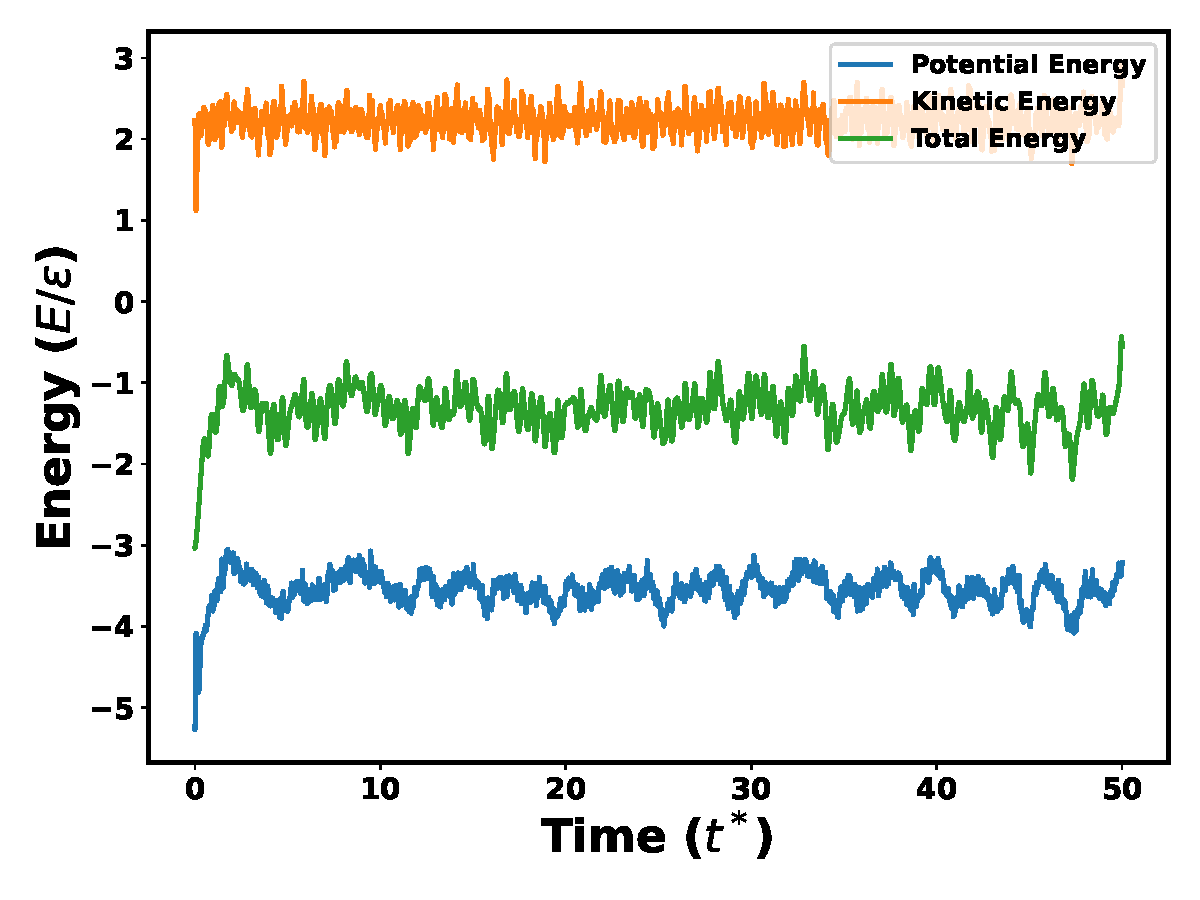
\includegraphics[width=\linewidth]{Figures/energy_vs_time_ts0.001.pdf}
\caption{Potential, kinetic, and total energy vs time.}
\end{subfigure}
\vspace{0.2cm}

\begin{subfigure}{0.8\linewidth}
\centering
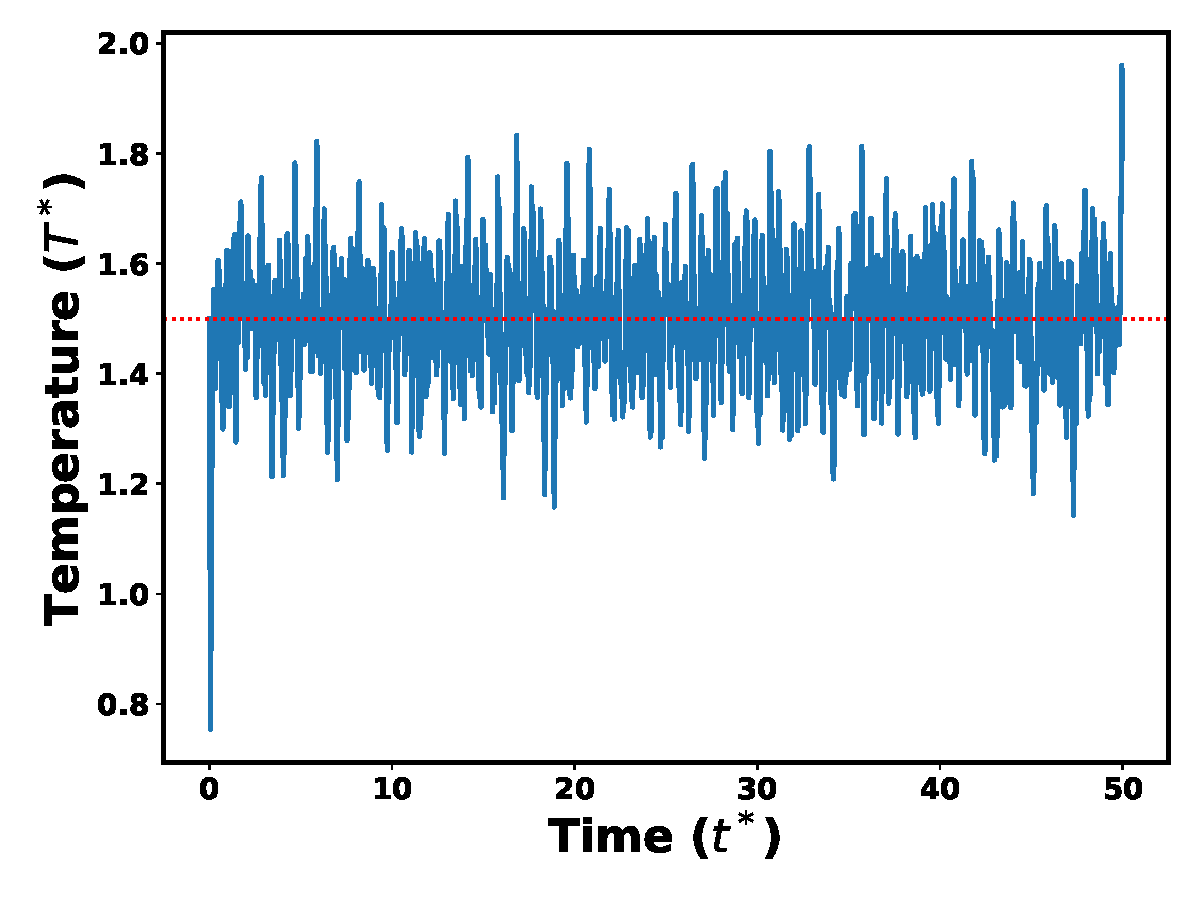
\includegraphics[width=\linewidth]{Figures/temperature_vs_time_ts0.001.pdf}
\caption{Temperature vs time ($T^*=1.5$).}
\end{subfigure}
\vspace{0.2cm}

\begin{subfigure}{0.8\linewidth}
\centering
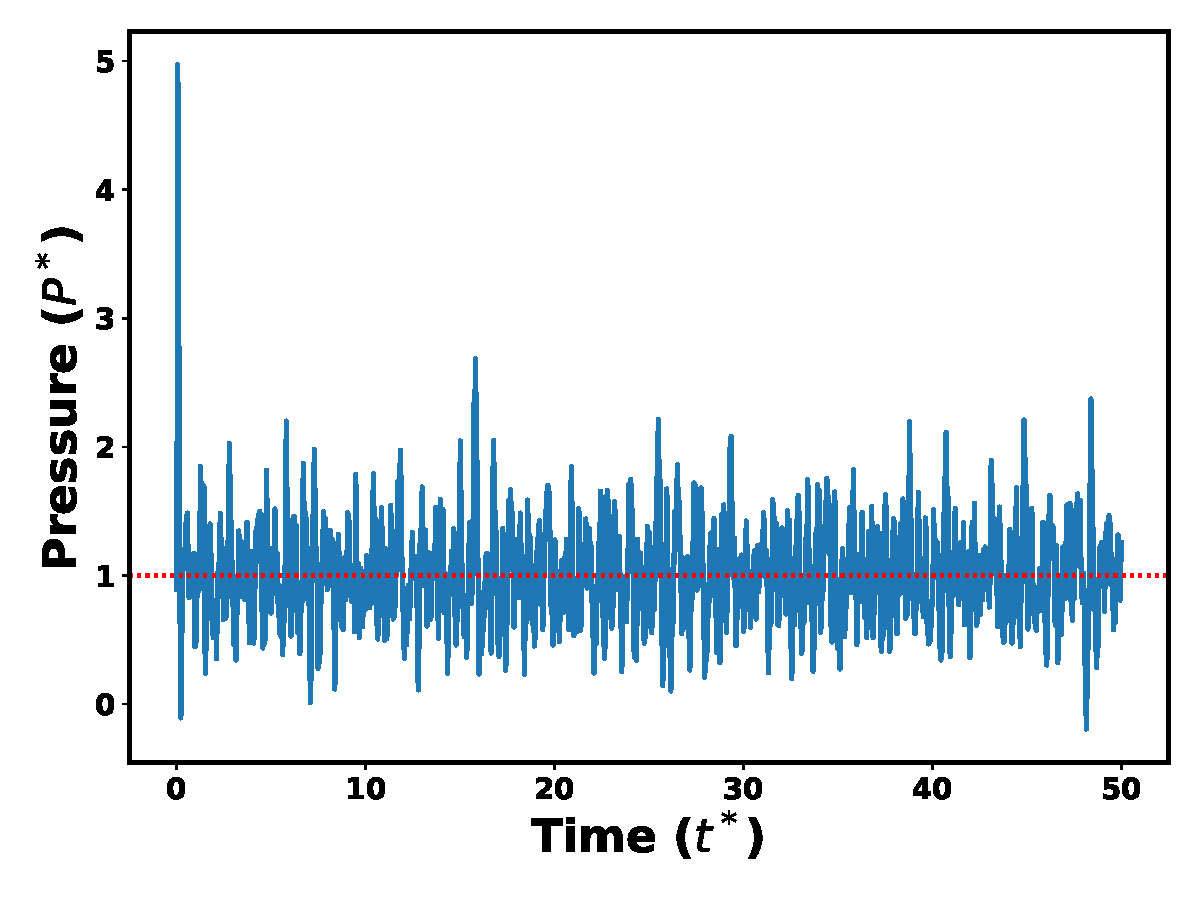
\includegraphics[width=\linewidth]{Figures/pressure_vs_time_ts0.001.pdf}
\caption{Pressure vs time ($P^*=1$).}
\end{subfigure}

\caption{Thermodynamic properties of the system during the NPT simulation with timestep $0.001$, where $T^*$ and $P^*$ is set to 1.5 and 1, respectively.}
\label{fig:equilibration}
\end{figure}


\subsubsection*{Make a single plot which shows the energy vs. time for the timesteps you have simulated [2].}
\begin{figure}[H]
    \centering
    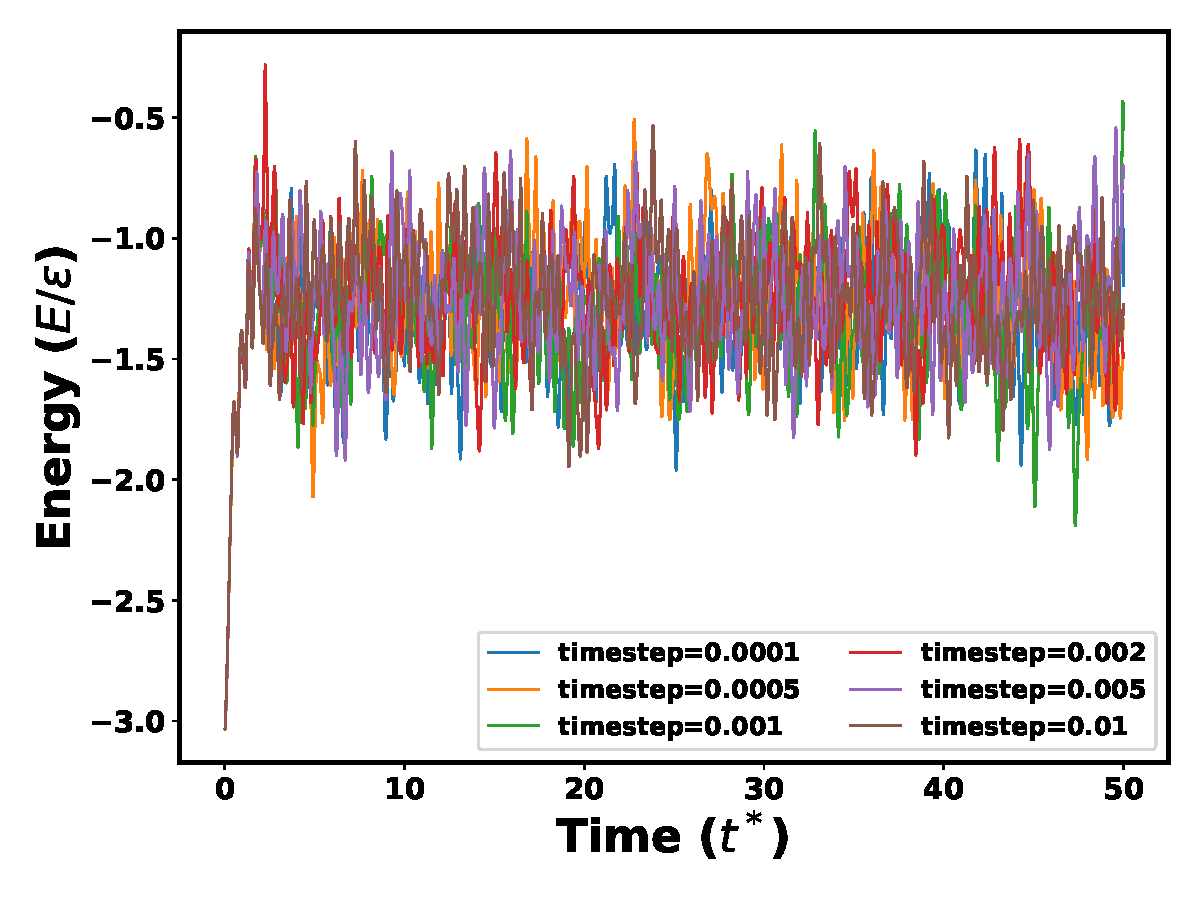
\includegraphics[width=0.9\linewidth]{Figures/energy_vs_time_different_ts.pdf}
    \caption{Total energy as a function of simulation time for NPT simulations with different timesteps. After equilibration, the energy fluctuates around a stable mean value for all tested timesteps, indicating numerical stability.}
    \label{fig:energy_vs_time_different_ts}
\end{figure}

\subsubsection*{Of the timesteps that you used, which timestep will you use for subsequent simulations and why? [6]}
\begin{figure}[H]
    \centering
    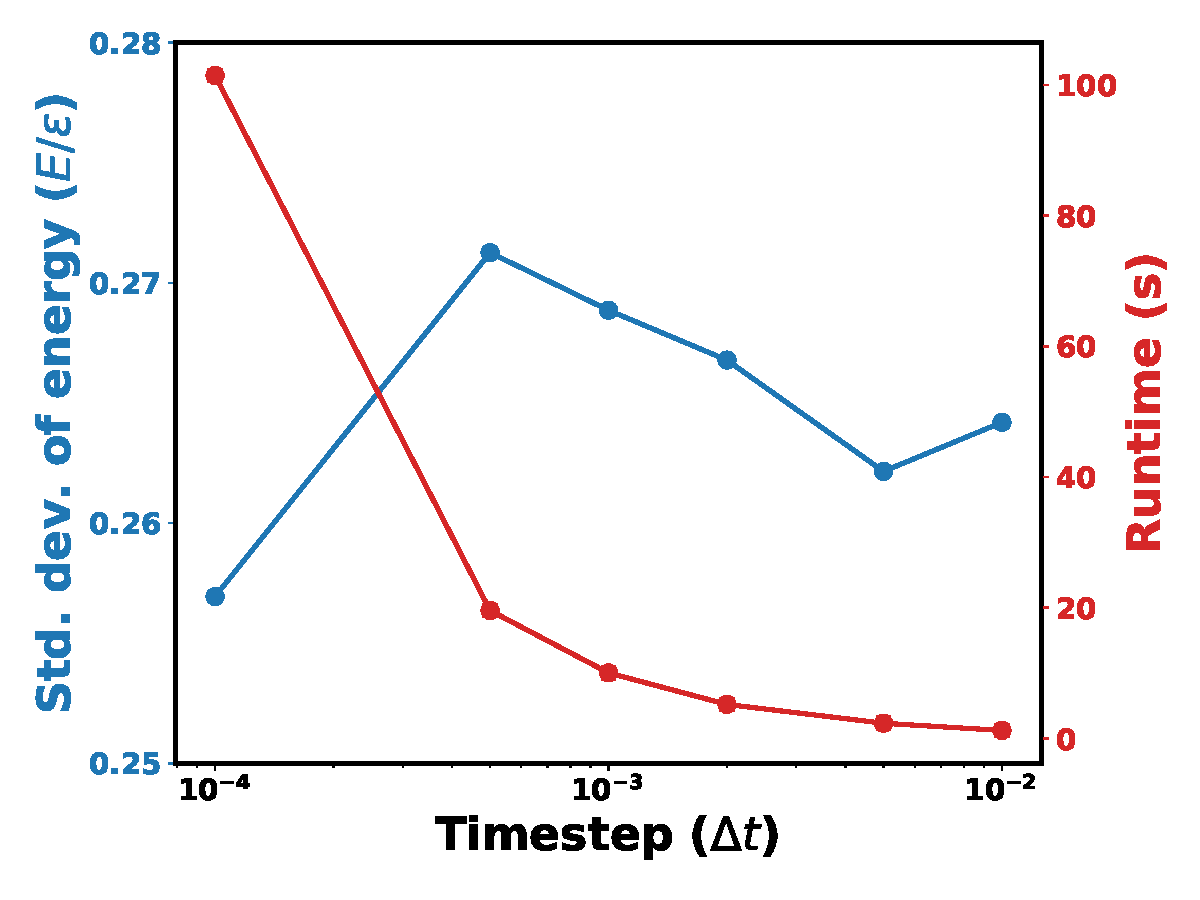
\includegraphics[width=0.9\linewidth]{Figures/timestep_stability_runtime.pdf}
    \caption{Standard deviation of the total energy (blue, left axis) and simulation runtime (red, right axis) as a function of integration timestep. The energy fluctuations remain similar across the tested timesteps, indicating numerical stability, while the computational runtime decreases rapidly with increasing timestep.}
    \label{fig:timestep_comparison}
\end{figure}

The standard deviation of the energy and total simulation runtime for the simulation with different timesteps are shown in Fig.~\ref{fig:timestep_comparison} (with $x$-axis plotted in log scale). It is found that while standard deviation remains similar, the total runtime decreases approximately inversely proportional to the timestep. Timestep $\tau= 0.001$ was therefore selected for subsequent simulations, as it provides good compromise between numerical stability and computational efficiency. Reducing the timestep further would only give minimal improvement with substantial increase in the runtime.

Physically, the timestep is the internal of physical time over which the equations of motion are integrated during the simulation. The unit of timestep $\tau$ is defined as:~\cite{frenkel2023understanding}
\[
\tau=\sqrt{\frac{m\sigma^2}{\varepsilon}}.
\]
At each timestep, the forces of the atoms are calculated, and positions and/or velocities are updated discretely. $\tau$ represents the time between two successive updates of the state of the system. Hence if the timestep is too large, the force calculations would become inaccurate, and the simulation is no longer valid physically. This effect is especially significant for LJ system, as it has a very strong repulsive term at short distances (e.g., at $r=0.9\ \sigma$, the LJ potential is already $5\ \varepsilon$). Therefore, the timestep must be small enough to \textit{resolve} the motions of the atoms.

On the other hand, if the timestep is too small, though the integration becomes highly accurate and the system becomes stable, the simulation becomes very compuatationally expensive.


\subsection{Running simulations under specific conditions}
\subsubsection*{Plot the density as a function of temperature for both pressures that you simulated. Include a line corresponding to the predictions made by the ideal gas law. [3]}
\begin{figure}[H]
    \centering
    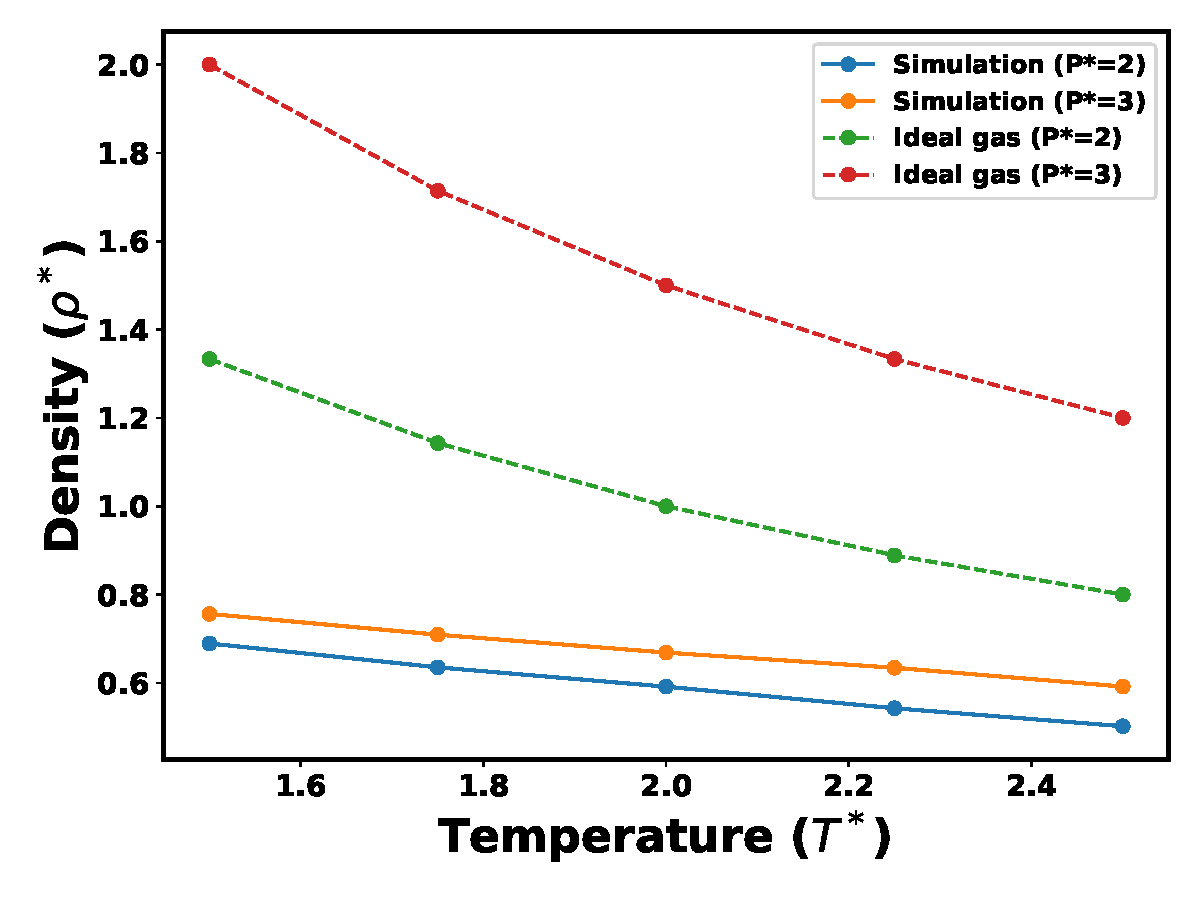
\includegraphics[width=1\linewidth]{Figures/density_vs_temperature_pressure.pdf}
    \caption{Density as a function of temperature for LJ simulations at pressures $P^*=2$ and 3 and temperatures $T^*=1.5,\ 1.75,\ 2,\ 2.25,\ 2.5$. The simulated densities are significantly lower than those predicted by the ideal gas law due to intermolecular interactions and excluded volume effects present in the LJ potential.}
    \label{fig:density_vs_temperature_pressure}
\end{figure}
\subsubsection*{How do your results compare to the ideal gas law? Do deviations increase/decrease with temperature and pressure? Explain. [7]}

Ideal gas law gives $PV=Nk_BT$ and therefore
\[
\rho=\frac{P}{k_BT}.
\]
Using the reduced unit, where $P^*=P\sigma^3\varepsilon^{-1}$, $T^*=k_BT\varepsilon^{-1}$, and $\rho^*=\rho\sigma^3$, this becomes
\[
\rho^*=\frac{P^*}{T^*}.
\]

Compared with the ideal gas prediction, the simulations yield significantly lower densities at the same temperature and pressure. This deviation arises because the ideal gas law neglects intermolecular interactions and assumes point-like particles, whereas the LJ potential includes both repulsive and attractive interactions. The repulsive core introduces excluded volume effects, while the attractive interactions reduce the effective pressure of the system compared with an ideal gas.

As the temperature increases, the deviation from ideal-gas behaviour
decreases. At higher temperatures the kinetic energy dominates over the
interparticle potential energy, so the system behaves more like an ideal gas.

In contrast, the deviation increases with pressure. At higher pressure the particles are forced closer together, making intermolecular interactions and excluded volume effects more significant.

This trend is consistent with the results shown in
Fig.~\ref{fig:density_diff_vs_temperature_pressure}, where the deviation is
largest at low temperature and high pressure.
\begin{figure}[H]
    \centering
    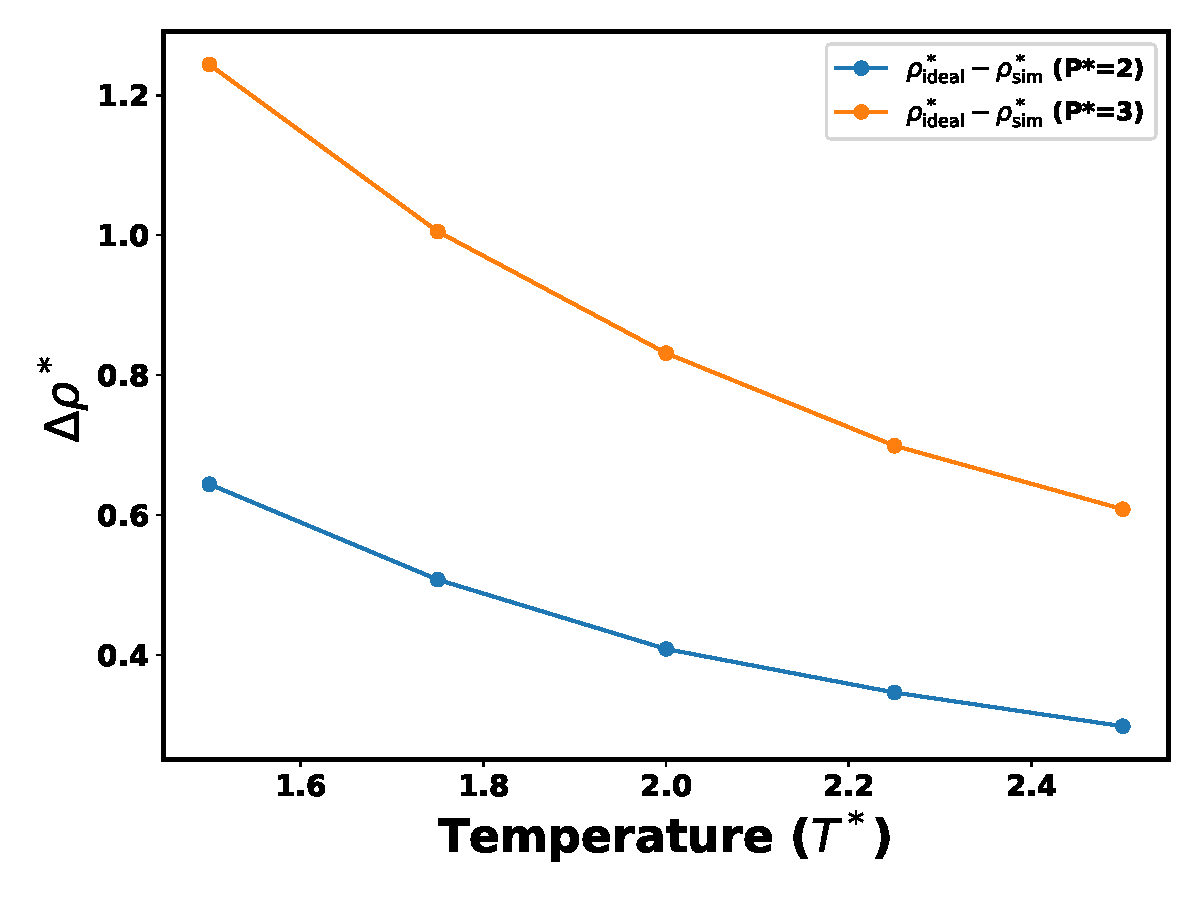
\includegraphics[width=1\linewidth]{Figures/density_diff_vs_temperature_pressure.pdf}
    \caption{Deviation of the simulated density from the ideal-gas prediction as a function of temperature at two pressures. The deviation decreases with increasing temperature and increases with pressure.}
    \label{fig:density_diff_vs_temperature_pressure}
\end{figure}

\subsubsection*{Do you expect your simulation results to be in better or worse agreement with the Van der Waals equation of state? Why? [3]}

The Van der Waals equation of state has the form
\[
(P+\frac{aN^2}{V^2})(V-Nb)=RT,
\]
where $a$ is attraction parameter, which corrects the attractive forces between particles, and $b$ is the excluded volume parameter, which corrects the finite size of molecules.

Compared to the ideal gas law, the two parameters introduced in the equation take the potential energy and particle volume into account, thereby the deviations could be reduced to a large extent, resulting in better agreement with MD simulation using LJ potential.

\subsection{Structural properties and the radial distribution function}
\subsubsection*{Briefly explain what a Radial Distribution Function is. What is the relationship between the coordination number and RDF? [2]}
Radial distribution function (RDF, $g(r)$) describes the probability of finding a particle at a distance $r$ from a reference particle relative to that of an ideal gas at the same density. It therefore characterises the spatial correlations and local structure of a system.

The coordination number ($n$) indicates the average number of neighbouring particles that can be found within the first coordination shell of the reference particle. Mathematically, it is obtained by integrating the RDF as~\cite{hines1985determination}:
\[
n=4\pi\rho\int_0^{r_{\text{min}}}r^2g(r)\ dr,
\]
where $\rho$ is the average density of the particles and $r_{\text{min}}$ is the position of first minimum of $g(r)$.

\subsubsection*{Plot the RDFs for the three systems. [2]}
\begin{figure}[H]
    \centering
    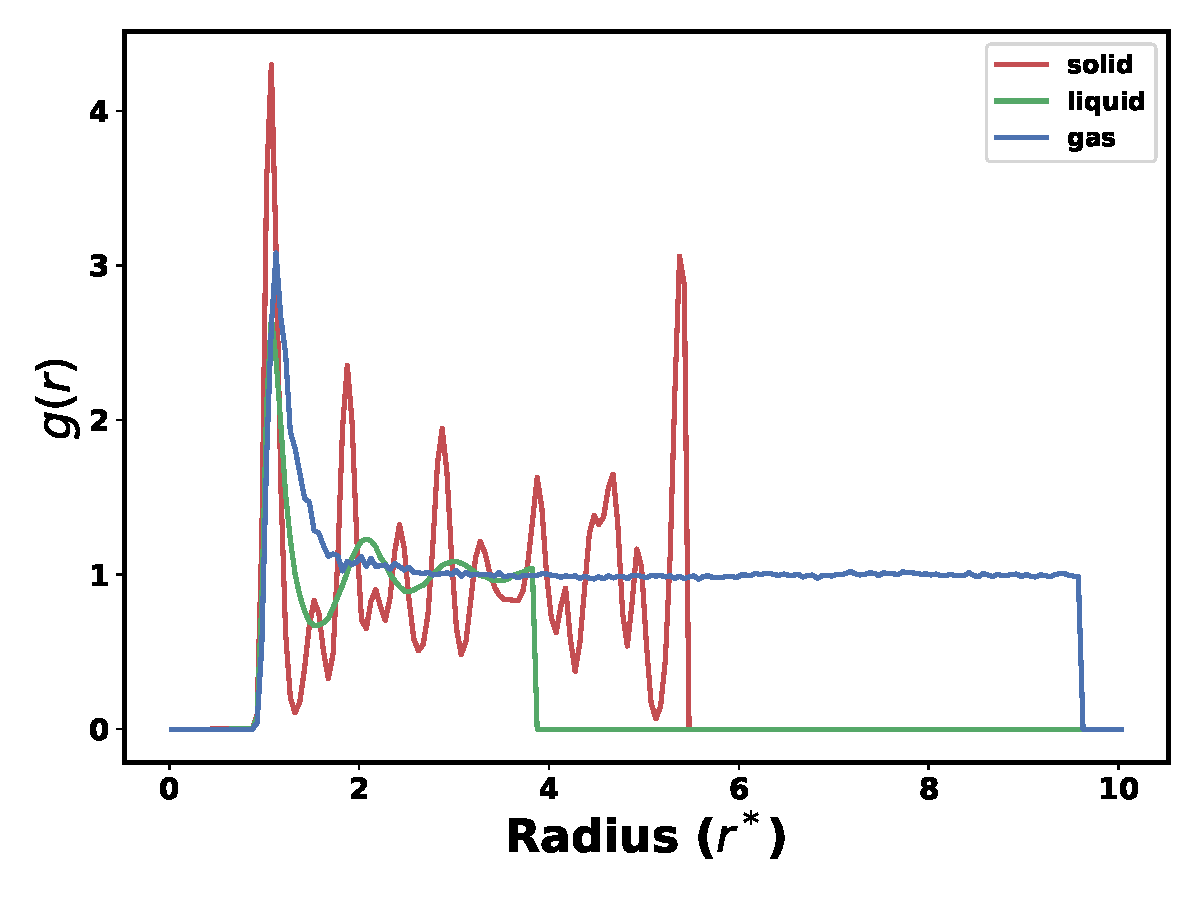
\includegraphics[width=1\linewidth]{Figures/rdf_states.pdf}
    \caption{Radial distribution functions $g(r)$ for the solid (FCC), liquid, and gas phases of the LJ system.}
    \label{fig:rdf_states}
\end{figure}

\subsubsection*{Discuss qualitatively the differences between the three RDFs, and what this tells you about the structure of the system in each phase. [5]}

The RDF of the solid phase displays multiple sharp peaks up to approximately $r^*=6$, reflecting the long-range periodic structure of the FCC lattice. 

The liquid phase exhibits a strong first peak and damped oscillations corresponding to short-range order. 

It is found that both the solid and liquid phases are cut off at a certain radius, illustrating the finite size of the simulation box and the maximum distance over which the radial distribution function is computed.

The gas phase RDF has a similar first peak to those of solid and liquid phase, after which it approaches $g(r)=1$, consistent with negligible spatial correlations. 

\begin{figure}[H]
    \centering
    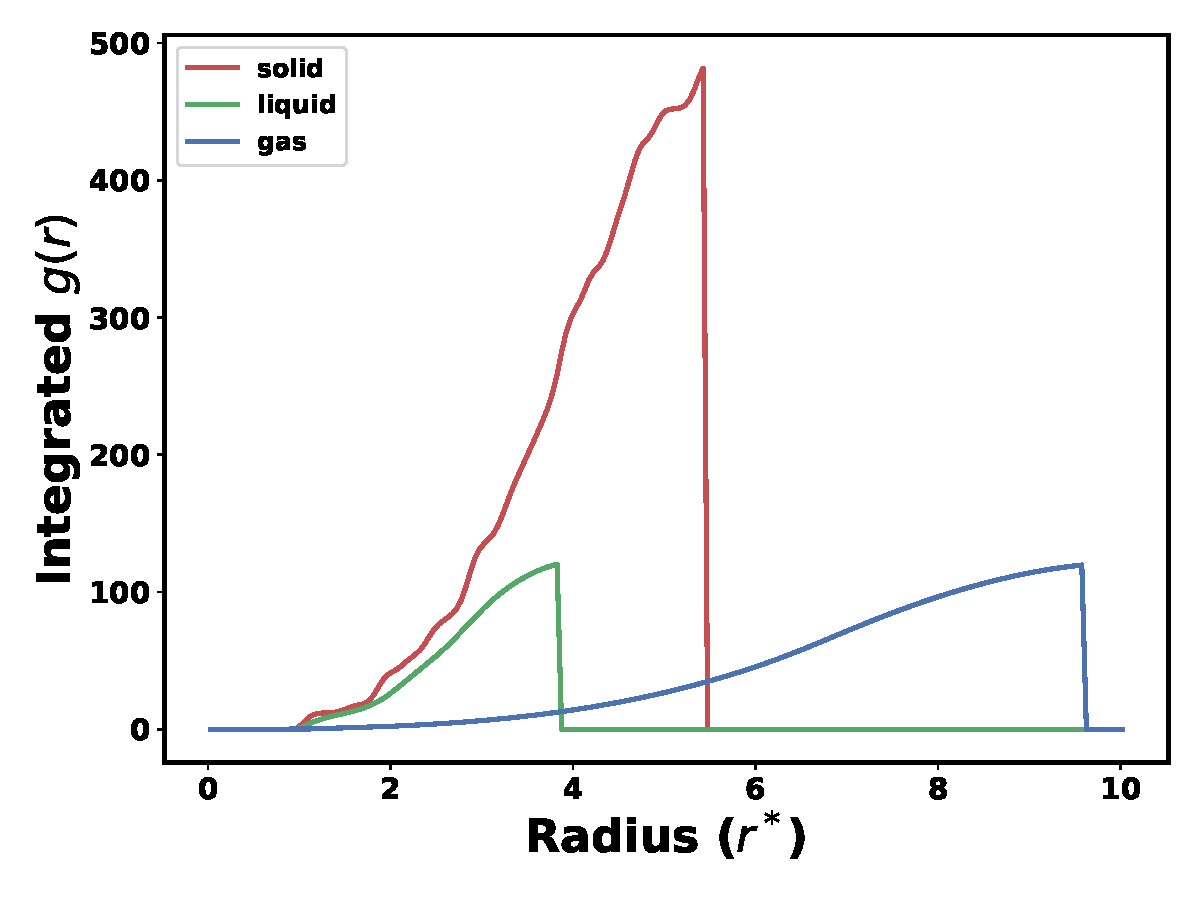
\includegraphics[width=1\linewidth]{Figures/rdf_integrated_states.pdf}
    \caption{Integrated radial distribution functions for the solid (FCC), liquid, and gas phases of the LJ system. The integrated $g(r)$ represents the cumulative number of particles within a distance $r$ from a reference particle.}
    \label{fig:rdf_int_states}
\end{figure}

Quantitative analysis of the RDF curves reveals the value of first $r_\text{min}$ (i.e., first coordination sphere) and the coordination number of each state (Table~\ref{tab:cn_states}). Simulation of the FCC solid yields a coordination number of 12.08, in excellent agreement with the theoretical value of 12. A similar coordination number with larger first coordination sphere is found for the liquid phase simulation, indicating the retention of short-range packing to a large extent. However, from Fig.~\ref{fig:rdf_states}, the damped oscillations after the first $r_{\text{min}}$ demonstrates the lack of long-range order. The first $r_{\text{min}}$ for gas is the highest among all, with significantly lower coordination number. This is consistent with the much lower density of the system, aligning with the weak and broad RDF curve and the nature of gas. Overall, the RDF clearly distinguishes the structural characteristics of the three phases, where the progressive reduction in structural order from solid to liquid to gas is directly reflected in the corresponding RDF profiles.

\begin{table}[H]
\centering
\caption{First minimum of the radial distribution function and corresponding coordination numbers for the three phases.}
\label{tab:cn_states}
\begin{tabular}{lccc}
\toprule
 & Solid & Liquid & Gas \\
\midrule
First $r_{\min}^*$ & 1.33 & 1.53 & 1.68 \\
$n$ & 12.08 & 12.05 & 1.39 \\
\bottomrule
\end{tabular}
\end{table}



\subsubsection*{In the solid case, illustrate which lattice sites the first three peaks correspond to [2]. What is the lattice spacing [1]? What are the coordination number for each of the first three peaks [1]?}
Let $a$ denote the cubic lattice parameter, then the first three peaks, i.e., the first three coordination shell distances are:
\[
r_1=\frac{a}{\sqrt2},\qquad r_2=a,\qquad r_3=\sqrt{\frac{3}{2}}a.
\]
The the corresponding lattice sites for the first peak include:
\[
\left(0,\frac{a}{2},\frac{a}{2}\right),\qquad \left(\frac{a}{2},0,\frac{a}{2}\right),\qquad \left(\frac{a}{2},\frac{a}{2},0\right),
\]
and symmetry-equivalent points. The coordination number of the first peak is 12. The lattice spacing can be obtained from the first peak position as
\[
a=\sqrt{2}\,r_1 .
\]
From the RDF, the first peak occurs at $r_1^*=1.33$, corresponding to
\[
r_1 = 1.33\,\sigma .
\]
Therefore,
\[
a=\sqrt{2}\times1.33\,\sigma = 1.88\,\sigma \quad \text{(to 3 s.f.)}.
\]
The the corresponding lattice sites for the second peak include:
\[
\left(a,0,0\right),\qquad \left(0,a,0\right),\qquad \left(0,0,a\right),
\]
and symmetry-equivalent points. The coordination number of the second peak is 6.

The the corresponding lattice sites for the third peak include:
\[
\left(a,\frac{a}{2},\frac{a}{2}\right),\qquad
\left(\frac{a}{2},a,\frac{a}{2}\right),\qquad
\left(\frac{a}{2},\frac{a}{2},a\right),
\]
and symmetry-equivalent points. The coordination number of the third peak is 24.

\begin{table}[H]
\centering
\caption{Radial positions of the first three RDF shell minima and the corresponding coordination numbers for the FCC solid from the simulation.}
\label{tab:fcc_shells}
\begin{tabular}{lccc}
\toprule
 & First shell & Second shell & Third shell \\
\midrule
$r_{\min}$ & 1.33 & 1.68 & 2.08 \\
$n$ & 12.08 & 5.95 & 25.91 \\
\bottomrule
\end{tabular}
\end{table}

From Table~\ref{tab:fcc_shells}, it is found that the simulation reproduces the expected coordination numbers of an FCC lattice. The first three coordination shells yield approximately 12.08, 5.95, and 25.91 neighbours, which are in good agreement with the theoretical values of 12, 6, and 24 for an ideal FCC structure.

\subsection{Dynamical properties and the diffusion coefficient}

\begin{figure}[H]
    \centering
    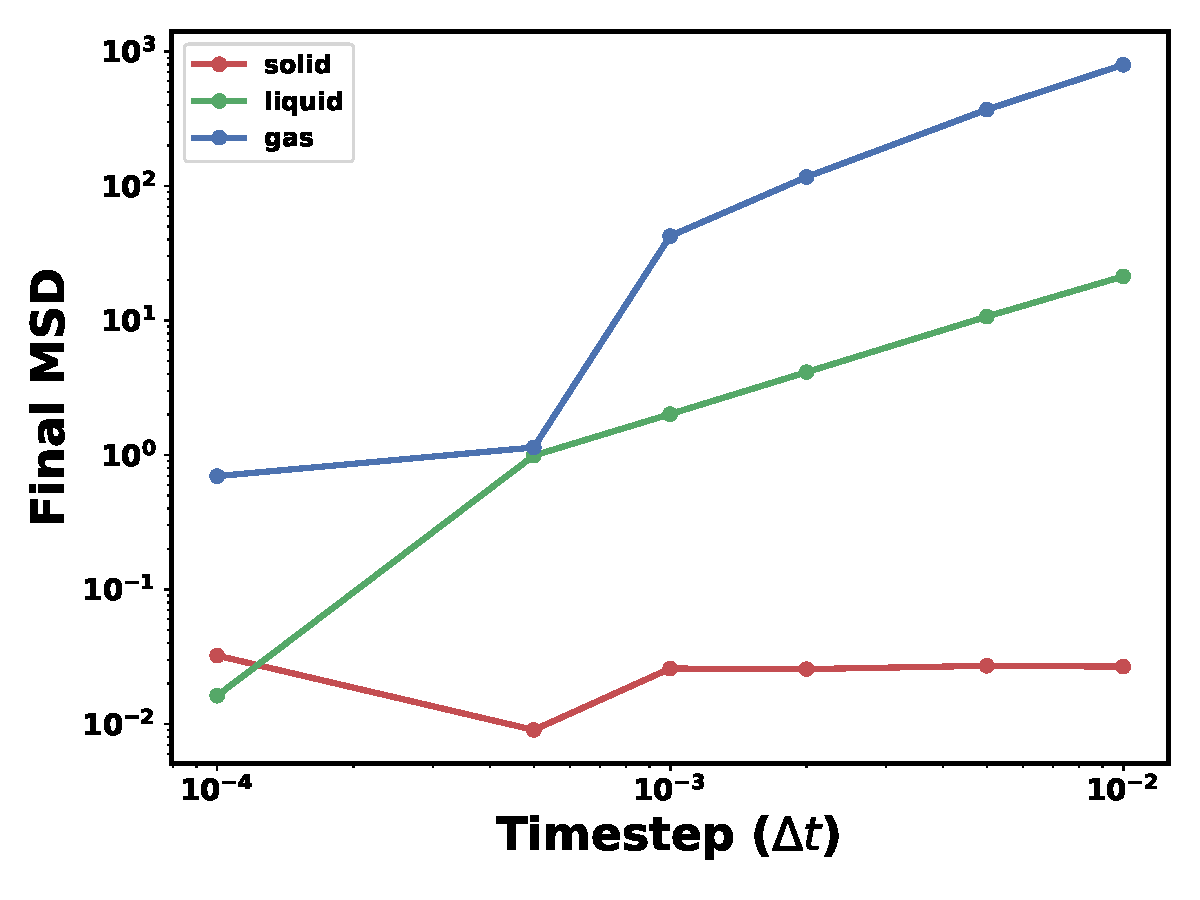
\includegraphics[width=1\linewidth]{Figures/final_msd_vs_timestep.pdf}
    \caption{Mean squared displacement (MSD) as a function of timestep obtained from the molecular dynamics simulations.}
    \label{fig:final_msd_vs_ts}
\end{figure}


\begin{figure}[H]
    \centering
    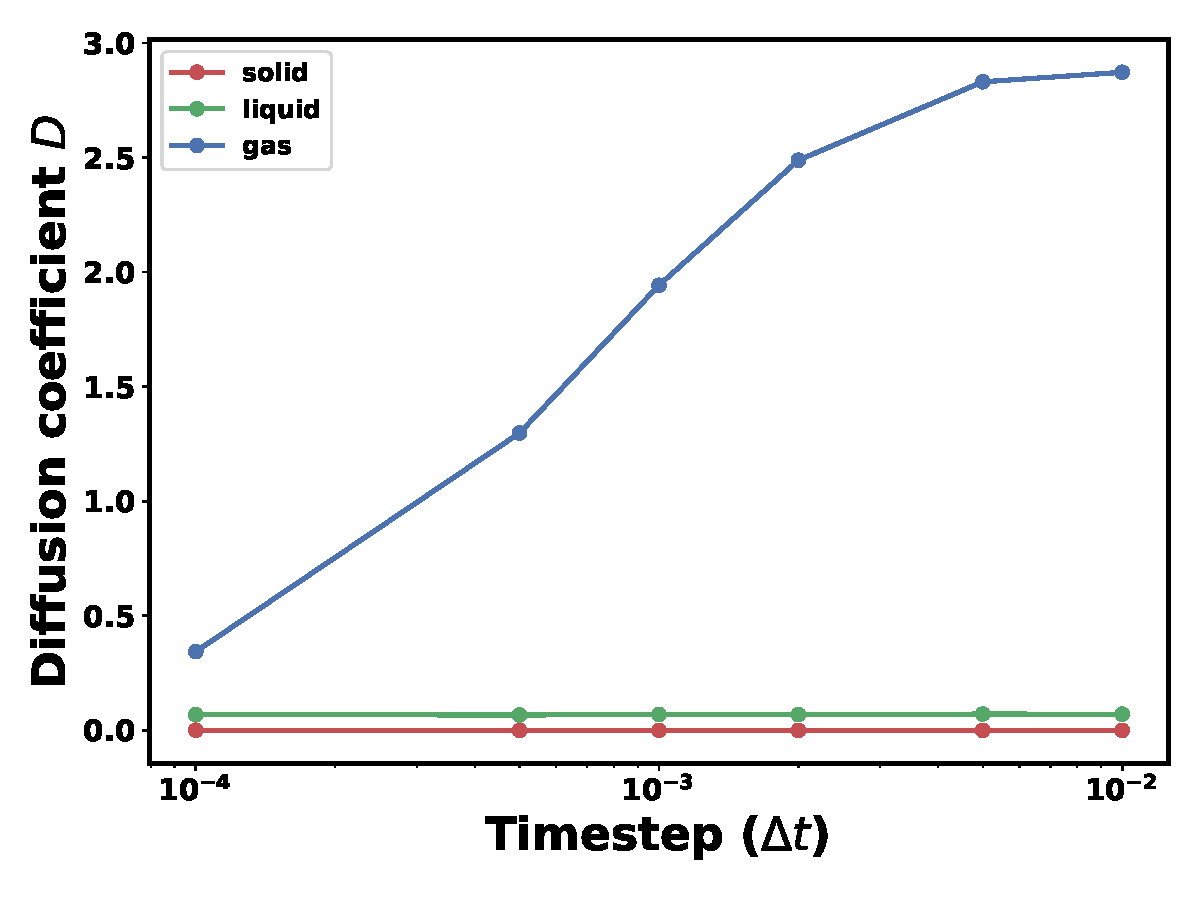
\includegraphics[width=1\linewidth]{Figures/D_vs_timestep.pdf}
    \caption{Diffusion coefficient $D$ as a function of timestep for the simulated systems. The diffusion coefficient is calculated from the slope of the mean squared displacement (MSD) using the Einstein relation $D=\frac{1}{6}\frac{d}{dt}\langle r^2(t)\rangle$. The results illustrate the distinct dynamical behaviour of the solid, liquid, and gas phases.}
    \label{fig:D_vs_ts}
\end{figure}

\begin{table}[H]
\centering
\caption{Effective diffusion coefficients estimated from the slope of the MSD curves. Since the simulation timestep for the one-million-atom trajectories is not available, the values are reported in units of simulation steps and should be interpreted qualitatively.}
\label{tab:diffusion_coefficients}
\begin{tabular}{lc}
\toprule
Phase & Effective diffusion coefficient $\tilde{D}$ \\
\midrule
Solid  & $-1.0\times10^{-5}$ \\
Liquid & $1.78$ \\
Gas    & $61.66$ \\
\bottomrule
\end{tabular}
\end{table}
% =========================================================
% 3. Conclusions (~20%)
% =========================================================
\section{Conclusions} % ~20\% of total marks, limit to ~1.5 page

\subsubsection*{In this lab, you have used the Lennard-Jones potential exclusively. Give one example of a system that can be described well using only LJ potentials. What additional elements would you need to add to the interaction potential to model a molecule, e.g. water? [6]}

Nobel gases atoms (e.g., Ar, Ne) can be described well with only LJ potentials due to their spherical, monoatomic and chemically inert nature~\cite{lenhard2024history}. There are no strong directional interactions or covalent bonds present in the interaction of nobel gas atoms. Instead, the interactions are dominated only by attractive London dispersion force and the short-range repulsive force arising from the Pauli exclusion principle (when overlap of electron clouds takes place when they are too close), both of which are captured by the expression of LJ potential. Therefore, the LJ potential provides a good estimation of their intermolecular interactions.

When modelling a more complex molecule, e.g, water, since each atom now has a positive or negative charge, the Coulombic electrostatic interactions must be taken into consideration:
\[
U_{\text{coulombic}}=\sum_{i<j}\frac{q_i q_j}{4\pi\varepsilon_0 r_{ij}}.
\]
In addition, the chemical bond stretches may be treated as a harmonic oscillator to account for the vibrations of the chemical bond:
\[
U_{\text{bond}}=\frac{1}{2}k_r(r-r_0)^2,
\]
and the bond angles can be maintained using an angle bending potential:
\[
U_{\text{angle}}=\frac{1}{2}k_\theta(\theta-\theta_0)^2.
\]
These refinements, along with the LJ potential terms shall give a better model when predicting the interactions of molecules as the polarity and molecular structure are taken into account.

\subsubsection*{What cut-off have you been using in your simulations? What are the advantages and disadvantages for using a shorter/longer cut-off? [3]}
The LJ potential can be truncated at certain cutoff distances by refining the equation as:
\[
U(r) =
\begin{cases}
4\varepsilon \left[ \left(\dfrac{\sigma}{r}\right)^{12}
- \left(\dfrac{\sigma}{r}\right)^6 \right], & r \le r_c, \\[6pt]
0, & r > r_c .
\end{cases}
\]

The input files used different LJ cutoffs for different tasks. A cutoff of 2.5$\sigma$ is used for thermodynamic calculations and structural calculations such as densities, energies and RDFs, while a larger cutoff of 3.2$\sigma$ is adopted for transport properties such as diffusion.

The selection of different cutoff distances reflects a trade-off between computational cost and accuracy. Using a shorter cutoff reduces computational cost because fewer pairwise interactions need to be calculated. However, truncating the potential too aggressively may neglect part of the long-range dispersion interactions arising from the $r^{-6}$ attractive term, which can introduce errors in thermodynamic and dynamical properties. Increasing the cutoff distance improves the accuracy of the potential by including more of these long-range interactions, but at the expense of higher computational cost.


\subsubsection*{In this lab you have investigated the properties of solids, liquids and gases. Would you observe a liquid phase (and by extension a critical point) if the LJ interaction strength, $\varepsilon$, is very weak? What interaction strength is required to generate a liquid phase? (Hint: to address this question you may want to revise the 2nd year Solids, Liquid and Interfaces lecture notes - see "Phase transitions of pure substances") [4]}

\subsubsection*{What are finite size effects? Do you think they are significant in the simulations you have performed? Why? [3]}

Finite size effects take place if the number of particles in our simulation is not sufficient to provide a statistically satisfactory description of the bulk environment of the system~\cite{reible2023finite}. 

Periodic boundary conditions can be applied to the system so that the simulation box is replicated infinitely in all directions. However, some residual finite size effects may still remain, particularly for properties involving long-range correlations or transport processes~\cite{allen2017computer}.

\begin{table}[H]
\centering
\caption{Numbers of atoms used in the simulations.}
\label{tab:atom_numbers}
\begin{tabular}{lccc}
\toprule
Simulation type & Gas & Liquid & Solid \\
\midrule
Diffusion & 800 & 800 & 3200 \\
RDF / NPT test & 125 & 125 & 500 \\
\bottomrule
\end{tabular}
\end{table}

In this study, the number of atoms used for diffusion calculations is sufficiently large to approximate bulk behaviour and reduce finite size effects. The systems used for the RDF and NPT tests are smaller, which may introduce greater statistical fluctuations of long-range correlations. However, these system sizes should still be adequate for capturing the qualitative structural and thermodynamic behaviour of the phases, and therefore finite size effects are expected to be limited in the context of the present study~\cite{frenkel2023understanding}.

\subsubsection*{Algorithms such as SHAKE and RATTLE are widely used to model molecular systems as they allow MD simulations to be performed while fixing bond lengths. Why is this desirable? [4] (Hint: think about the timestep.)}

    
% =========================================================
% References
% =========================================================
%\section*{References}
{\small
\setlength{\bibsep}{0pt}
\bibliographystyle{achemso}
\bibliography{references}
}

\section*{Supporting Information} 
\setcounter{figure}{0}
\renewcommand{\thefigure}{S\arabic{figure}}
\setcounter{table}{0}
\renewcommand{\thetable}{S\arabic{table}}

\begin{figure}[H]
\centering

\begin{subfigure}{\linewidth}
\centering
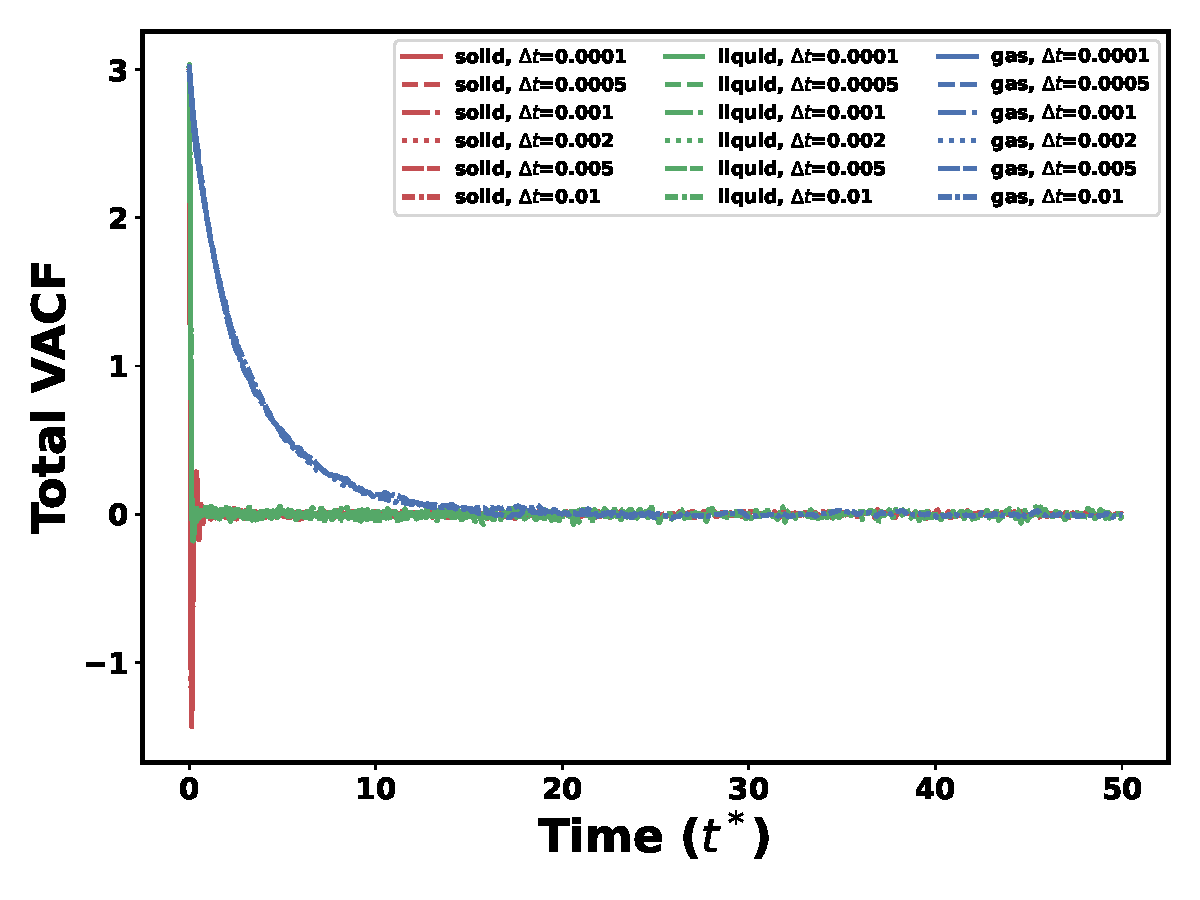
\includegraphics[width=\linewidth]{Figures/vacf_vs_time.pdf}
\caption{Total velocity autocorrelation function (VACF) as a function of reduced time $t^*$ for the solid, liquid, and gas phases at different timesteps $\Delta t$.}
\end{subfigure}

\begin{subfigure}{1\linewidth}
\centering
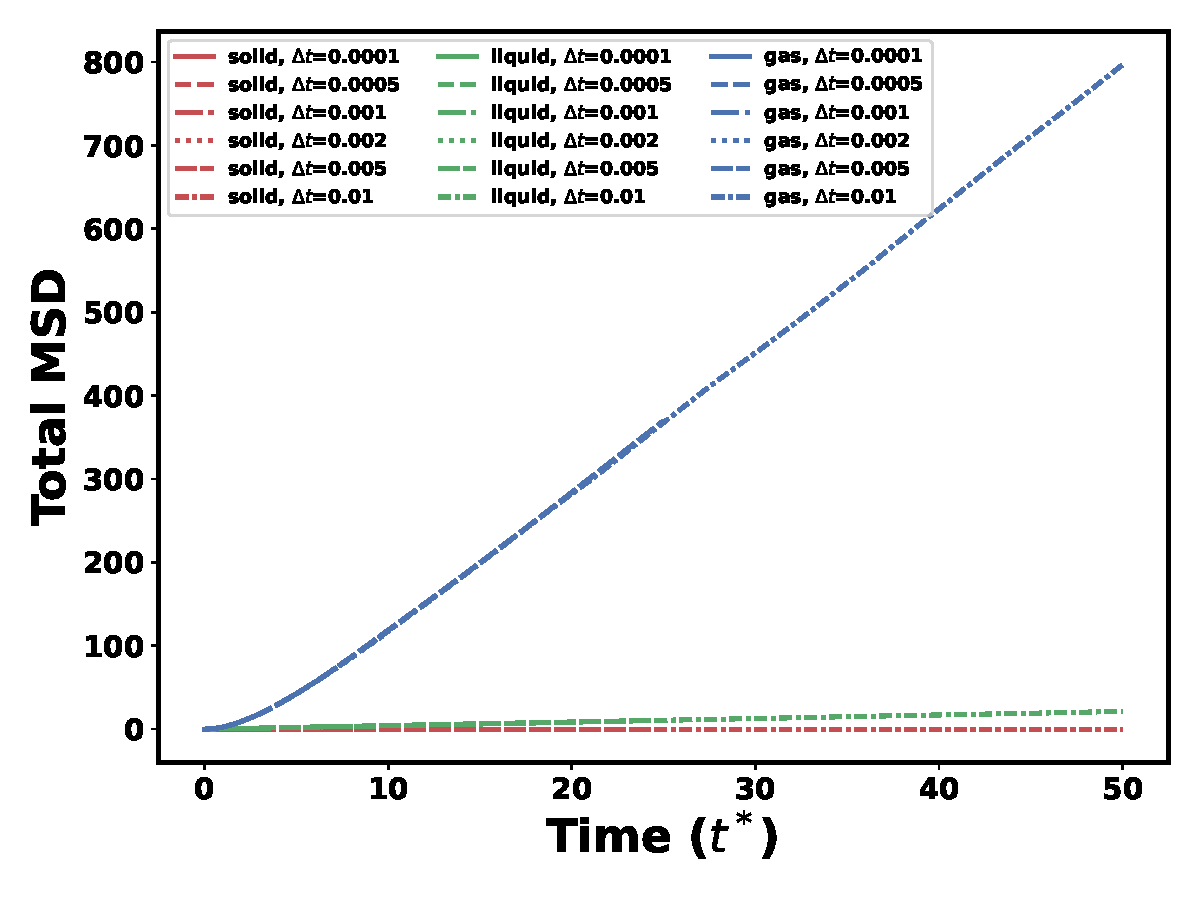
\includegraphics[width=\linewidth]{Figures/msd_vs_time.pdf}
\caption{Mean squared displacement (MSD) as a function of reduced time $t^*$ for the solid, liquid, and gas phases at different timesteps $\Delta t$.}
\end{subfigure}


\caption{Dynamical properties of the Lennard--Jones system obtained from molecular dynamics simulations at different timesteps.}
\end{figure}

\end{document}